%%%%%%%%%%%%%%%%%%%%%%%%%%%%%%%%%%%%%%%%%
% Peking Univ. Physical Review (cn)
%
% LaTeX Template
% Version 2.1
% Release 03/19/18
%
% Original author:
% Mathias Legrand (legrand.mathias@gmail.com) 
%
%%%%%%%%%%%%%%%%%%%%%%%%%%%%%%%%%%%%%%%%%
%
%----------------------------------------------------------------------------------------
%	PACKAGES AND OTHER DOCUMENT CONFIGURATIONS
%----------------------------------------------------------------------------------------
%\RequirePackage{times}      % Loads the Times-Roman Fonts
%\RequirePackage{mathptmx}   % Loads the Times-Roman Math Fonts
\let\nofiles\relax % 加入这一行即可,关键的一行
\documentclass[10pt,a4paper,twocolumn]{PPRAcn} % Document font size

\usepackage[UTF8]{ctex}
\usepackage[english]{babel} % Specify a different language here - english by default
\usepackage{lipsum} % Required to insert dummy text. To be removed otherwise
\usepackage{bm,caption,textcomp,subfigure,float}
\usepackage[keeplastbox]{flushend}
\usepackage{geometry}
\newgeometry{top=28mm,bottom=25mm,left=20mm,right=25mm}

\newcommand{\upcite}[1]{\textsuperscript{\textsuperscript{\cite{#1}}}}

%----------------------------------------------------------------------------------------
%	COLUMNS
%----------------------------------------------------------------------------------------

\setlength{\columnsep}{7.0mm} % Distance between the two columns of text
\setlength{\fboxrule}{0.75pt} % Width of the border around the abstract
\setlength{\abovecaptionskip}{5pt}
\setlength{\belowcaptionskip}{0pt}

%----------------------------------------------------------------------------------------
%	COLORS
%----------------------------------------------------------------------------------------

\definecolor{color1}{RGB}{0,0,90} % Color of the article title and sections
\definecolor{color2}{RGB}{0,20,20} % Color of the boxes behind the abstract and headings

%----------------------------------------------------------------------------------------
%	HYPERLINKS
%----------------------------------------------------------------------------------------

\usepackage{hyperref} % Required for hyperlinks
\hypersetup{hidelinks,colorlinks,breaklinks=true,urlcolor=color2,citecolor=color1,linkcolor=color1,bookmarksopen=false,pdftitle={Title},pdfauthor={Author}}

%----------------------------------------------------------------------------------------
%	ARTICLE INFORMATION
%----------------------------------------------------------------------------------------

\newcommand{\keywordname}{Keywords} % Defines the keywords heading name
\captionsetup[figure]{name={图}}
\captionsetup[table]{name={表}}
\captionsetup{font={small}}
%\JournalInfo{Journal, Vol. XXI, No. 1, 1-5, 2013} % Journal information
%\Archive{Additional note} % Additional notes (e.g. copyright, DOI, review/research article)

\PaperTitle{用于玻色取样的自发参量下转换单光子源的优化(Optimizing spontaneous parametric down-conversion sources for boson sampling)} % Article title


\Authors{李明达\textsuperscript{1}} % Authors
\affiliation{
	\quad
	\textsuperscript{1}\textit{中国科学技术大学物理学院:学号PB18020616}
	\qquad
} % Author affiliation

\Abstract{
	\phantom{田田}本阅读报告首先调研了论文以外的一些知识点,从单光子源、HOM干涉实验、准相位匹配、自发参量下转换、非线性晶体到玻色取样,涵盖了读懂本论文所需要的所有量子光学与非线性光学知识。随后,笔者又采用一种相对于原论文更加有逻辑的方式来阐述该论文的脉络与思路,并给出这篇文章的结论——可以利用SPDC光子源实现“量子优越性”。最后,笔者从自己作为一个量子光学学习者的观点,来论述我对这篇文章的心得体会。
}


\Keywords{\phantom{田田}量子光学、非线性光学、单光子源、量子计算、玻色取样、自发参量下转换、非线性晶体、数值模拟} % 如不需要关键词可直接删去花括号中内容


 %这是标题,作者和摘要(关键词)

%----------------------------------------------------------------------------------------

\begin{document}

\flushbottom % Makes all text pages the same height

\maketitle % Print the title and abstract box

%\tableofcontents % Print the contents section

\thispagestyle{empty} % Removes page numbering from the first page

%----------------------------------------------------------------------------------------
%	ARTICLE CONTENTS
%----------------------------------------------------------------------------------------

\section{调研一、单光子源以及$g^{(2)}$}

\subsection{什么是单光子源?}

既然我们要调研单光子源,那么首先要知道什么是单光子源。那么什么是单光子源呢?有的人会说,取一个激光光源,然后持续衰减,使它在给定的时间范围内,光子的平均数量达到1或小于1,就可以搞成一个“单光子源”了。但是,如果稍有一些量子光学知识就会发现,其实这是错误的。这是因为激光发出的光,无论怎么衰减,最终都是相干态,而不是单光子态,所以无论再怎么衰减也不是真正单光子源。

真正的单光子源,是指其产生的光场的态,是单光子态$|1\rangle$

\subsection{单光子源有哪些?[1]}

常见的单光子源主要有SPDC单光子源、基于Atoms-Ions的单光子源、以及量子点单光子源、NV色心单光子源,以及四波混频单光子源。我们将逐一介绍[1]:

1.  SPDC source:这个是这篇论文用到的光子源,被称为自发参量下转换光子源,是我们目前最广泛使用和流行的产生单光子的方法。
它的产生是由于一个二阶非线性光学过程,其中一个高能量泵光子,在一个非线性介质的存在,自发地产生两个低能量光子,称为信号光子和空闲光子。如图\ref{fig:SPDC1}所示。

\begin{figure}[ht]
	\centering
	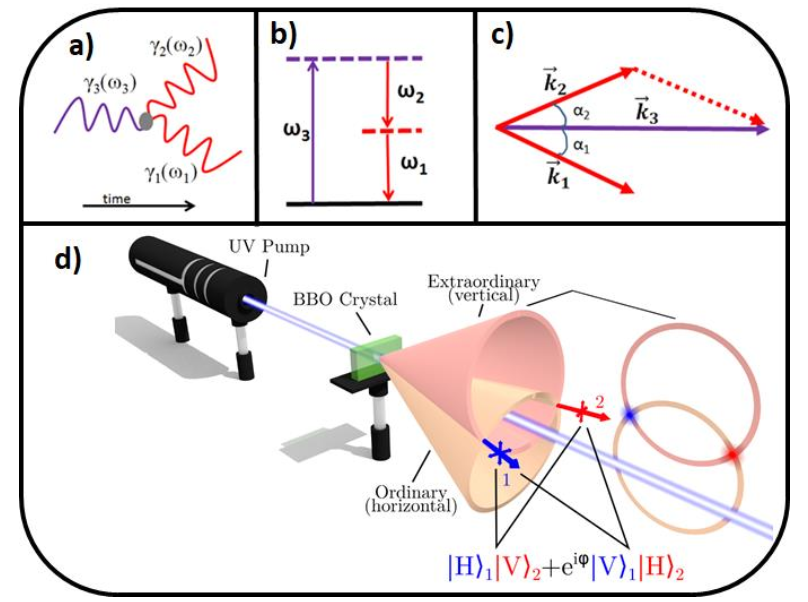
\includegraphics[scale=0.2]{pic/SPDC1}
	\caption{SPDC过程示意图}
	\label{fig:SPDC1}
\end{figure}

这个过程是自发的(由量子真空场产生),并且是参数化的(介质的初始和最终量子力学状态是相同的,光子能量总是守恒的),也是信号频率和空转频率总是低于泵浦频率的下转换的一个例子。后面我会提到,SPDC过程遵循能量守恒和动量守恒,这两者统称为相位匹配条件。SPDC过程可用于预先提出的方案中产生单光子。

由于这两个光子是同时产生的,探测到一个就预示着另一个的出现,所以可以用于产生可预示的单光子。

它的优点是:可以亮度很高,保真度很高,光子的全同性很好;缺点是:产生光子是概率的、效率较低。

2.  四波混频:在这种情况下,两个泵浦光子在非线性介质中转换为一个信号光子和一个闲散光子。这个过程满足相位匹配条件。

与SPDC不同的是,四波混频一般只出现在包含波导的集成光学结构中,而SPDC既可以发生在bulk上,也可以发生在像空腔和波导这样的受限几何中。由于相互作用模式的数量较少,波导源通常比bulk source具有更高的对产生率. 四种基于波混频的光子源报道了亮度在0.855 MHz左右。
目前纠缠保真度的记录是$99.7\%$。

3.  基于原子离子的单光子源:通过冷原子技术把原子/离子束缚在一个固定的位置,利用原子能级之间的跃迁实现单光子源。而且,由于purcell效应,如果腔与原子耦合得比较好,则该单光子源则有很大的几率以腔模初射,这就保证了不同光子之间的全同性。如图\ref{fig:qdot}

4.  基于量子点得单光子源:所谓量子点实际上就是“人工原子”,事实上,这是未来最有前途的光子源之一,在未来的发展和应用中具有很大的潜力。
量子点是直径在210nm范围内的半导体材料的微小粒子或纳米晶体。由于它们的原子状离散能谱,它们被称为人工原子。当光脉冲照射时,量子点及其附近的电子从价带跃迁到导带,从而形成电子-空穴对,然后迅速松弛到最低能级如图\ref{fig:qdot}。

\begin{figure}[ht]
	\centering
	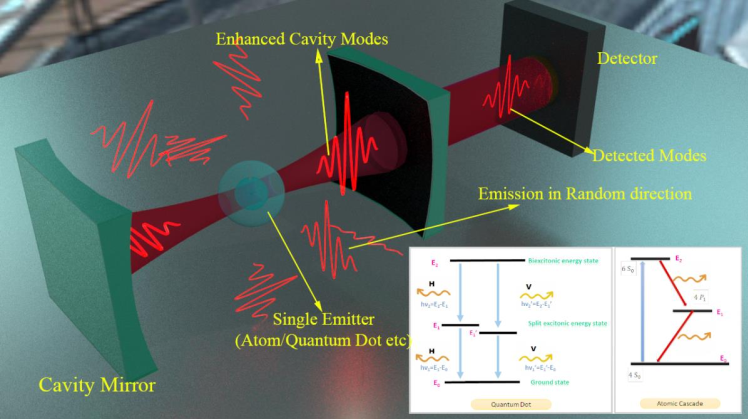
\includegraphics[scale=0.2]{pic/qdot}
	\caption{原子/离子/量子点过程示意图}
	\label{fig:qdot}
\end{figure}

根据数量的不同,我们可以从激子,双激子和多激子的状态观察到重组,这是指剩下的电子-空穴对的数量。虽然所有这些跃迁具有不同的能量,原则上可通过光谱滤波作为单光子的发射器,但双激子跃迁和激子跃迁是最常用的.

5.  NV色心:另一项即将到来的、有前途的技术是基于碳中的色心。在金刚石结构中,缺少碳原子会导致缺陷。用一个氮原子代替这些缺陷,而不用碳原子代替另一个缺陷。这就是所谓的金刚石中的氮空位(Nitrogen-Vacancy)色心。类似地,其他原子也可以取代氮,从而产生一系列钻石色心。

\textbf{以上所有的单光子源可以概括到一下这个图中,如图\ref{fig:singlephotonsources}}

\subsection{如何判断单光子性?——$g^{(2)}$[2,3]}
单光子性可以通过HB-T干涉仪来检验,通过测$g^{(2)}$函数来判断是否是单光子。在延迟时间为0的时候,二阶相关度可以写成\[g^{(2)}(0)=\frac{P_{12}}{P_1P_2}\]
一个典型的实验结构以及预期结果如图\ref{fig:g2}所示。

\begin{figure}[ht]
	\centering
	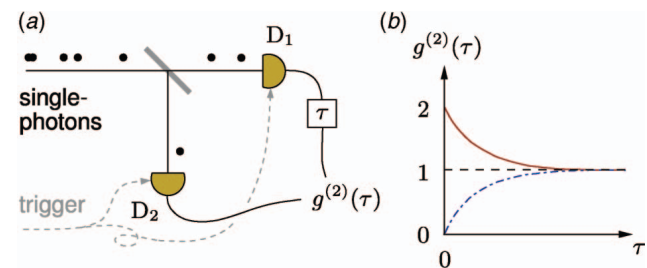
\includegraphics[scale=0.25]{pic/g2}
	\caption{典型的HB-T干涉仪(a)以及相应的结果(b)}
	\label{fig:g2}
\end{figure}

如果是单光子,那么测得的$g^{(2)}(0)=0$,所以判断一个单光子源的单光子质量如何只需要检验这个等式即可。


\section{调研二、衡量全同光子的标准——HOM干涉[2,3]}

HOM干涉是量子光学里一个非常重要的干涉,也是张老师在量子光学课讲过很多次的一个知识点,但我调研了一个更加“量子光学”的方法——光子波包法,我把它概括如下:

我们假设经过分束器之前的光模场为$a_1^\dagger$和$a_2^\dagger$,经过分束器之后变为$a_3^\dagger$和$a_4^\dagger$. 对k模式的光场,我们写出它的模式函数:
\[\zeta_k(t)=\epsilon_k(t)exp(-i\phi_k(t))\]
如图\ref{fig:hom}所示。

\begin{figure}[ht]
	\centering
	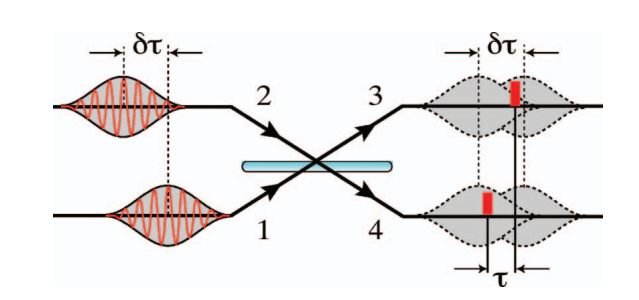
\includegraphics[scale=0.25]{pic/hom}
	\caption{HOM干涉仪的图示}
	\label{fig:hom}
\end{figure}


\begin{figure*}[ht]
	\centering
	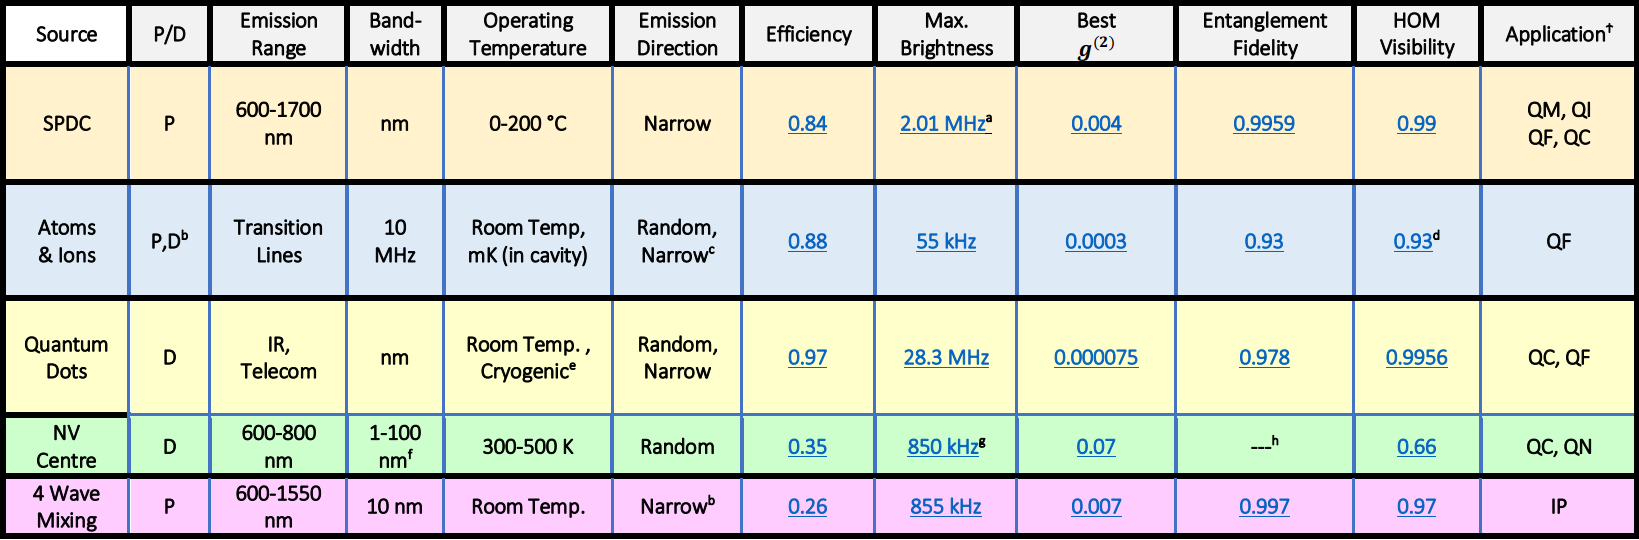
\includegraphics[scale=0.25]{pic/singlephotonsources}
	\caption{各种各样的单光子源参数对比}
	\label{fig:singlephotonsources}
\end{figure*}


我们可以算出在3,4处同时检测到光子的概率,这里我直接给出结果:
\[P_{3,4}(t_0,\tau)=\frac{1}{4}|\zeta_1(t_0+\tau)\zeta_2(t_0)-\zeta_2(t_0+\tau)\zeta_1(t_0)|^2\]

如果两个光子不是全同的,则当$\tau\neq0$时,一定存在$P_{34}\neq0$的点,比如,在图\ref{fig:hom1}中,我给出一个其他都相同,但波包持续时间不同的情况。

\begin{figure}[ht]
	\centering
	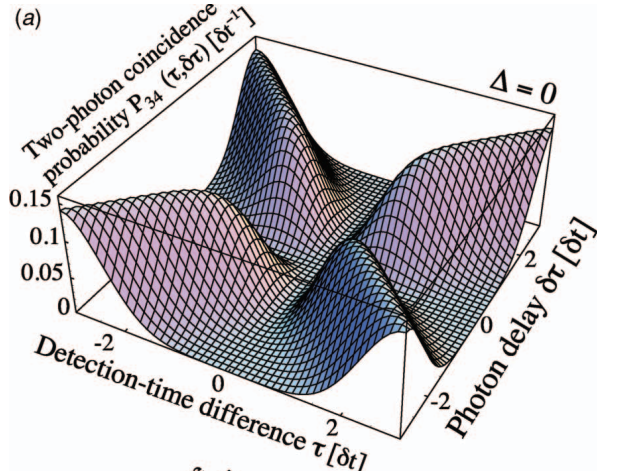
\includegraphics[scale=0.25]{pic/hom1}
	\caption{如果两个光子“颜色”相同(频率相同)但波包持续时间$\delta\tau$不同,在$\tau\neq0$时,可以看到$P_{34}\neq0$,这与我们期待的结果相符}
	\label{fig:hom1}
\end{figure}

通过这种方法,我们可以去判断两个光子是否是全同的。


\section{调研三、(准)相位匹配与自发参量下转换}
\subsection{相位匹配与准相位匹配[4]}
这里的准相位匹配(QPM—Quasi-phase-matching)要区别双折射相位匹配(BPM—birefringent phase matching),后者是用基态波和二阶谐波折射率相同而做到的。提到了BPM,这里我要多说一句关于相位匹配:BPM是只对于SHG中,它是指折射率相同;而在和频差频中,靠的是相位匹配,这里的相位匹配不再局限于双折射,它满足的方程是:        ,或者说“动量守恒”的方程。

下面我们研究研究SHG的相位关系,特别是$△k≠0$的时候。为了显示结果,我们把上一章最后一个方程,用复数线积分的图形表示,即所谓的相量图——phasor diagram(此相量非彼向量)。

这个图的构建是通过把每个小区域的积分,当成对每一小段复数域路径的求和。如图\ref{fig:QFM1}所示:

\begin{figure}[ht]
	\centering
	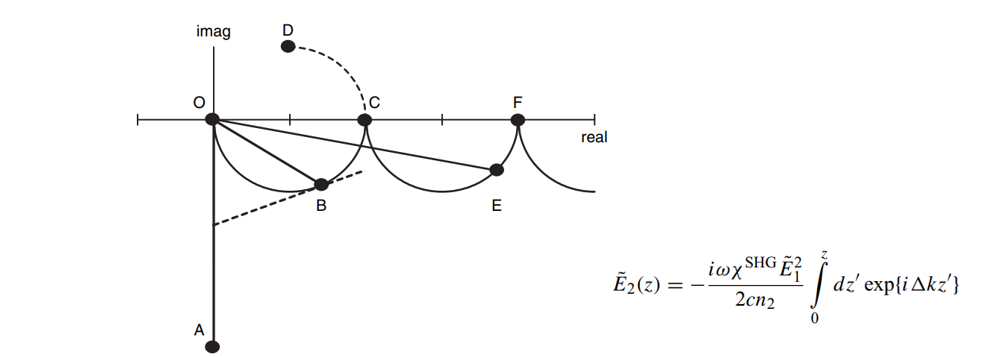
\includegraphics[scale=0.2]{pic/QFM1}
	\caption{相量图——phasor diagram}
	\label{fig:QFM1}
\end{figure}

我把涉及到的一个公式和这个图组合在了一起。下面我们来看这图。
如果基态电场$\widetilde{E_1}$是实正数(那个公式里面的平方不是模),则可以看出$\widetilde{E_2}$是虚负的。所以当$△k=0$的时候,随着z的增加$\widetilde{E_2}$与z成平方增大,也就是成为OA直线,可见OA的长度正比于z的平方。(这里要说一下这个图的参数是z,也就是走的坐标距离。)
但是,如果有色散出现的话,这个相量图会变化成一条曲线。对于正常色散$(n2>n1)$,$△k>0$,这也就意味着图线会偏离OA,而像一个圆一样逆时针旋转到OB,但这个过程由于积分项纯粹是对于相位,所以OB的圆弧长度和OA还是相等(这个用复数模长为1的积分很好验证)。所以这只影响路径的形状,不影响路径长度。$\widetilde{E_2}$的模长(前面说的是路径长)也就是直线OB的长度,很容易看出来OB的圆心角是$△k\times z$,通过这个图也很容易看出来$OB=OC\sin{\frac{\triangle k\times z}{2}}$,在一个共振长度后,也就是$z=L_{cor}=\frac{\pi}{\Delta k}$的时候,曲线走到了C,这时候可以认为基态波和二阶谐波“同相”,因为$\widetilde{E_2}$的振幅最大。此后,如果不进行操作,他将会继续沿着D到达O. 
但这个图给我们提示了一种其他的可能性——如果在C点突然变号,那么路线将会走向E,F……然后振幅就变的越来越大……这可不可以也作为一种让二阶波展现出来的办法呢?
幸运的是,这在实验上可以被实现。通过一个由一系列非线性晶体片组成的晶体,每个晶体一个共振长度厚,然后交替晶体的方向相反。

这种方法被Armstrong, Bloembergen, Ducuing and Pershan提出。然而,过了很多年之后这才被用定期极化(periodic poling)稳定地实现。

这种方法QPM和BPM有很大不同,从相量图可以看出来,BPM就是OA,而QPM是圆弧上点到原点距离。

极化周期(poling period)被定义为一对板的厚度
$L_{pole}=2L_{coh}=\frac{2\pi}{\left|\triangle k\right|}$
实际上,只有几十微米,所以这些板很薄。

在QPM情况下的光强如图\ref{fig:QFM2}所示:

\begin{figure}[ht]
	\centering
	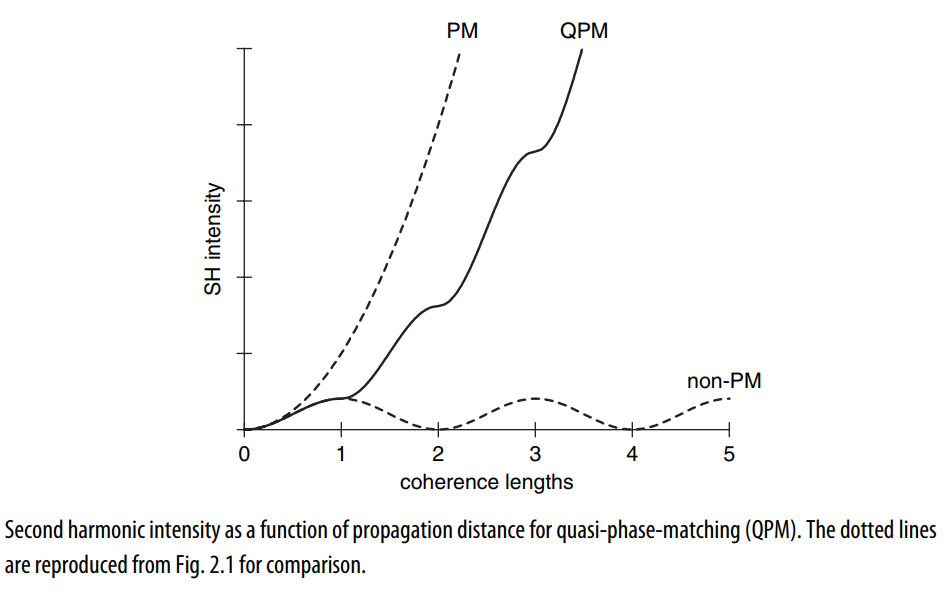
\includegraphics[scale=0.3]{pic/QFM2}
	\caption{在QPM情况下的光强}
	\label{fig:QFM2}
\end{figure}

需要说的是,这是因为这个图是关于光强而不是电场场强的,所以每个层高度不一样,是平方增加的。如果被画成电场强,每个是相等的。


最后考虑一下PM和QPM的比例,从相量图可以看到,当z很大的时候,场强比近似为$\frac{2}{\pi}\approx0.637$,所以光强比为$0.405$

这其实也让我有了一个新的想法(如右图):用一些△k相反的晶体拼成一个完整晶体,也就是,正常色散和非正常色散交替,不知道可不可行。

\subsection{自发参量下转换[5]}
有一种非线性晶体可以用来将光子分裂成一个光子对,原本的光子称为“泵浦光子”,光子对里的两个光子分别任意称为“信号光子”、“闲置光子”。按照能量守恒定律与动量守恒定律,光子对的总能量与总动量等于泵浦光子的能量与动量。

从能量守恒定律可以得到\[\hbar\omega_p=\hbar\omega_s+\hbar\omega_i\]

从动量守恒可以得到\[\vec{k_p}=\vec{k_s}+\vec{k_i}\]

其中,p、s、i分别为泵浦光子、信号光子、闲置光子的角频率,这两个条件合在一起称为相位匹配条件。这个过程如图\ref{fig:SPDC}所示。

\begin{figure}[ht]
	\centering
	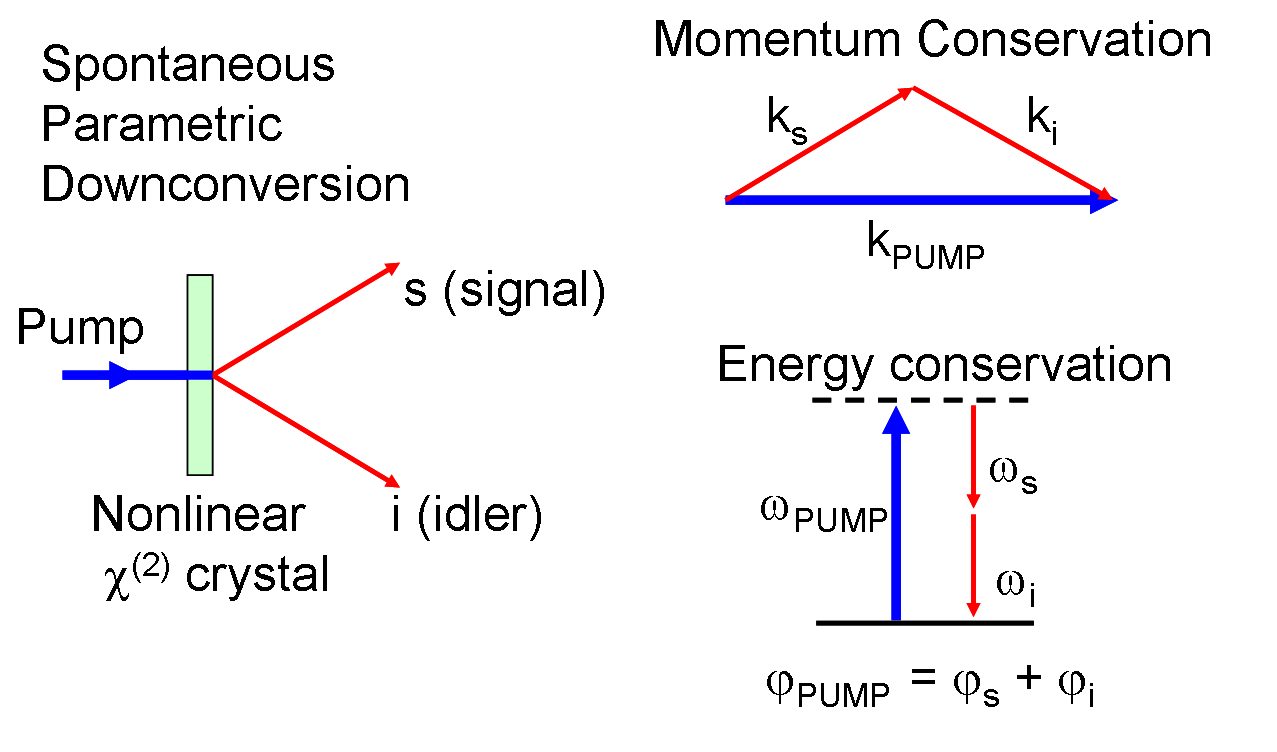
\includegraphics[scale=0.3]{pic/SPDC}
	\caption{过程示意图}
	\label{fig:SPDC}
\end{figure}

这两个关系式称为相位匹配条件。只有某些种类的非线性晶体能够达到这条件,例如,偏硼酸钡晶体或磷酸二氢钾晶体。

假若信号光子与闲置光子的共享同样的偏振,并且与泵浦光子相互垂直,则称此为第一型关联;假若信号光子与闲置光子的偏振相互垂直,则称此为第二型关联。相继发射的光子对彼此之间没有任何偏振关联。

自发参量下转换是由随机的真空涨落所激发,因此光子对被生成于随机时刻。转换效率很低,大约每$10^{12}$个入射光子会生成一个光子对。假若仪器探测到信号光子,则闲置光子必定也存在

\section{调研四、非线性晶体}
本论文主要讨论了三种非线性晶体:钛氧基磷酸钾(ppKTP)、β-硼酸钡(BBO)、磷酸二氢钾(KDP)

1.	钛氧基磷酸钾(ppKTP)[6]

KTP这种晶体在通信波长上具有对称群速度匹配特性,这个特性有利于获得纯态,因此是一种普遍的选择。同时,因为KTP源使用周期性的极化——准相位匹配,所以它的光子产生速率很高。此外,周期极化通过高斯变迹法实现了高斯型相位匹配函数

2.	β-硼酸钡(BBO)[7]

BBO晶体的特点是可以产生当前记录的光子数量,也能产生电信波长的光子。然而它有不对称的群速度匹配,这会导致降低光谱纯度。

3.	磷酸二氢钾(KDP)[8]

KDP源产生的光子在830nm左右,在没有滤波情况下,它可以产生已知的产生最高纯度的光子。

\section{调研五、玻色取样 \\ $(Boson$ $ sampling)^{[9]}$}

问题起源于2011年Aaronson和Arkhipov(AA)两人提出,使用Fock状态输入的被动线性光学干涉仪的操作不可能被经典计算机模拟[10]。也就是说,当线形变换的计算矩阵阶数较高时,我们可以用被动线性光学元件对结果进行取样,但通过经典的计算机却无法计算。

首先我们约定一下一个符号体系:

我们用vacuum state来表示$|0\rangle=\left[
 \begin{matrix}
   1 \\
   0
  \end{matrix}
  \right]$,用single photon state来表示$|1\rangle=\left[
 \begin{matrix}
   0 \\
   1
  \end{matrix}
  \right]$,一般的态可以写成$|\psi\rangle=c_0|0\rangle+c_1|1\rangle$. 那么如果把被动线性光学器件作用在不同模式的态中,其实也就相当于对这个态的系数进行矩阵变换,比如分束器就可以被描述为

$$
 B_{\theta,\phi}=\left[
 \begin{matrix}
   cos\theta & -e^{i\phi}sin\theta  \\
   e^{-i\phi}sin\theta & cos\theta 
  \end{matrix}
  \right]
$$

这时,玻色取样的问题可以概括如下:

我们从一个在m个模式中有n个单光子(m>n)的输入态开始,

\begin{align*}
|\psi_{in}\rangle
&=|1_1,...,1_n,0_{n+1},...,0_m\rangle\\
&=\hat{a_1}^\dagger...\hat{a_n}^\dagger|0_1,...,0_m\rangle
\end{align*}

在经过某种配置的一系列变换之后,这个态最后变成了\[|\psi_{out}\rangle=\Sigma_S\gamma_S|n_1^{(S)},...,n_m^{(S)}\rangle\]
其中S是指一个特定的配置,$n_{i}^{S}$是指在S配置下第i个模式中输出的光子数。以模式S输出的几率是$P_S=|\gamma_S|^2$,如图\ref{fig:BS}所示

\begin{figure}[ht]
	\centering
	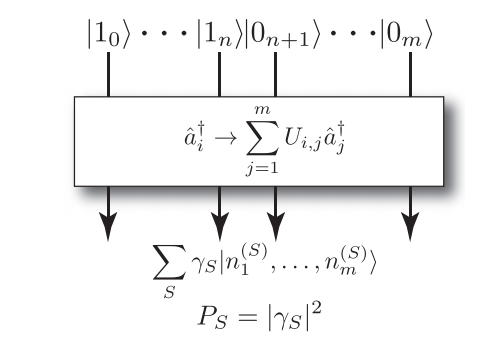
\includegraphics[scale=0.3]{pic/BS}
	\caption{玻色取样法图示}
	\label{fig:BS}
\end{figure}

理论上可以证明,\[\gamma_S=\frac{Per(U_S)}{\sqrt{n_1^{(S)}!...n_m^{(S)}!}}\]
其中$Per(U)$是指U的积和式。


比如,如果考虑1,2模式进入,2,3模式输出,如图\ref{fig:1223}所示

\begin{figure}[ht]
	\centering
	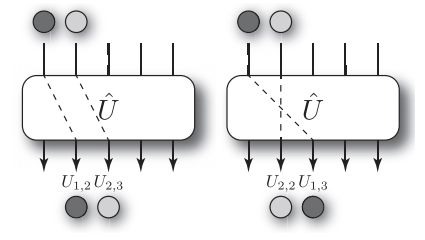
\includegraphics[scale=0.3]{pic/1223}
	\caption{从12模式进入,从23模式输出一共有两种,一种是直接通过,另一种是交换通过。}
	\label{fig:1223}
\end{figure}

那么此时振幅大小可以写成:

\begin{align*}
\gamma_{(1,2)-(2,3)}
&=U_{1,2}U_{2,3}+U_{1,3}U_{2,2}   \\
&= Per \left[\begin{matrix}
   U_{1,2} & U_{2,2}  \\
   U_{1,3} & U_{2,3}
  \end{matrix}
  \right]
\end{align*}

类似我们还可以考虑其他情况,如果是从(1,2)变成(4,4),重复对应的计算即可。

我们可以概括成以下的普遍情况,如果我们有n个光子,就会有n!种光子到达输出的方式(假设它们都到达不同的输出),每个振幅将一直与一个$n\times n$矩阵的积和式对应。计算积和式是一个有名的数学问题,最好的算法是Ryser的算法,需要$O(x^nn^2)$量级的计算量[11]。所以一旦矩阵阶数变大,用传统计算机做这个计算就变得不再可能(比如取50).

而玻色取样的方法是对量子系统做指数级的测量,这会大大体现量子计算的优势,也就是一个典型的体现“量子优越性”的办法。

这篇论文所讨论的,使用SPDC单光子源实现玻色取样法的方案如图\ref{fig:SPDCBS}所示。

\begin{figure}[ht]
	\centering
	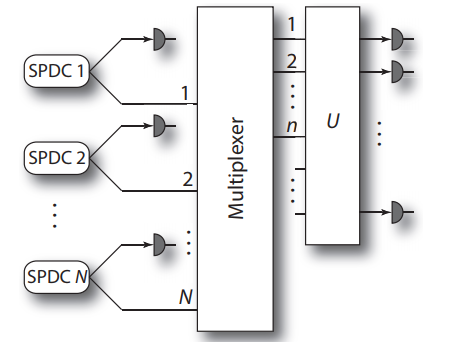
\includegraphics[scale=0.3]{pic/SPDCBS}
	\caption{使用SPDC单光子源实现玻色取样法的方案,其中我们需要N个SPDC单光子源。}
	\label{fig:SPDCBS}
\end{figure}


\section{为什么需要优化SPDC光子源?}
光量子信息处理发展到今天,已经取得了很大的进步,但人们一直追求突破,其中最重要的一个就是实现“量子霸权”(quantum supremacy),即:展示出量子计算机相对于经典超级计算机的优势。

当可以精确操纵的量子比特超过一定数目时,量子计算机在特定任务上的计算能力就能远超经典计算机。在量子计算的版图上,光子、电子、离子等微观粒子都被科学家用来尝试实现可能的计算方案。其中,线性光学量子计算(LOQC)是量子计算的方案之一。所谓线性光学量子计算,就是以光子作为载体,经过一个线性系统完成操作,输出计算结果。实现大规模比特的通用量子计算机目前看来还具有很苛刻的门槛,于是,科学家希望能够首先让量子计算在特定任务上表现出比经典计算机更卓越的能力。其中,一个叫做“玻色取样”(Boson Sampling)的问题吸引了科学家的关注。

根据Aaronson 和Arkhipov当年提出的论文 [10],玻色取样的核心思想是:n光子“玻色取样”的分布概率正比于n维矩阵积和式(Permanent)的模方,从计算复杂度的角度来看,积和式的求解难度是“$\#P-hard$” [11],当前经典最优算法需要O(n2n)步,随着光子数的增加求解步数呈指数上涨。对于这样一个经典计算P-complete困难的问题,在中小规模下就可以打败超级计算机。因此,“玻色取样”这个问题被量子计算领域的科学家盯上了,准备拿它小试牛刀,挑战经典计算机。

但是玻色取样的方法需要很多很多满足以下两个要求的光子:

1.	尽量无损

2.	几乎全同

自发参量下转换光子源(SPDC sources)是目前世界上最流行的光子源之一,所以本文就是为了优化SPDC光子源来实现前面所说的量子优势。

但是立马就来了第一个问题,传统的Boson Sampling随着光子数的增加会花费指数增长的时间,所以不是很合适,所以人们用Scattering Boson Sampling的办法替代了它。但此时仍然需要光子保持非常高的全同性,我们要如何才能让光子尽量全同呢?

其中一种很好办法是光谱过滤(spectral filtering),但却会产生另外一个问题——造成光子的损失,这违背了第一个要求:尽量无损。

所以这篇论文的目的就是,为了寻求“全同”与“无损”的平衡,在最好的平衡位置,证明这是有可能实现量子优势的。

本文主要讨论了三种非线性晶体:钛氧基磷酸钾(ppKTP)、β-硼酸钡(BBO)、磷酸二氢钾(KDP)




\section{本论文的理论模型与模拟方法}
这篇论文的计算,考虑共线配置下的高斯型脉冲泵浦的SPDC过程。并且这里做了一个假设:假设只存在一种空间模式,不考虑聚焦效应,并且我们忽略了高光子数态。
\subsection{1.SPDC光子源模型}

SPDC源的原理是通过自发参量下转换过程,把一个光子变成一对光子。SPDC过程可以从能量守恒$\hbar\omega_p=\hbar\omega_s+\hbar\omega_i$和动量守恒$\vec{k_p}=\vec{k_s}+\vec{k_i}$来理解,其中p代表pump光子,s代表signal光子,i代表idler光子,这个过程如图\ref{fig:SPDC1}所示[5]。


其中动量守恒的式子就是相位匹配的条件,一般情况下,在介质中,由于双折射现象,只有特定的波长组合能满足这俩条件,而这个组合也就是这个双光子态中,两个光子的频谱时间关联特性——这两个光子是有关联的,而关联越少,我们可以说这两个光子的谱纯度越高。从物理意义出发,谱纯度其实也就是光子的全同性。

我们常用Joint Spectral Intensity(JSI)来描述两光子的关联,数学表述是
\[JSA=f\left(\omega_s,\omega_i\right)=\alpha\left(\omega_s,\omega_i\right)\phi\left(\omega_s,\omega_i\right)\]

其中能量守恒和动量守恒各给出一个约束条件,分别是$\alpha\left(\omega_s,\omega_i\right)$和$\phi\left(\omega_s,\omega_i\right)$

为方便理解,图\ref{fig:JSI}是一个典型的JSI的图,其中图中的红色虚线是指我们接下来要讲的光谱过滤(spectral filtering)

\begin{figure}[ht]
	\centering
	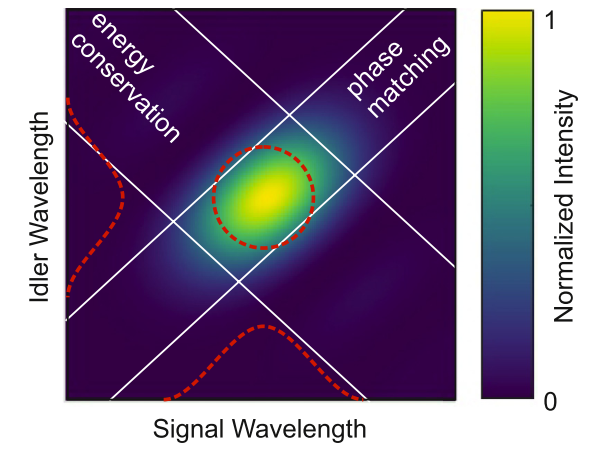
\includegraphics[scale=0.6]{pic/JSI}
	\caption{联合光谱强度(JSI)的一个例子。
红色虚线显示了信号和空闲光子的高斯滤波器。
对角白线表示满足相位匹配(能量守恒)的区域。}
	\label{fig:JSI}
\end{figure}

前面我们说了,在这个过程里,我们常用光谱过滤,那么为什么我们需要光谱过滤呢?

这是因为我们的目的是希望两个光子是全同的,所以这也就是说我们需要这两个光子的谱纯度非常高,所以也就需要这两个光子的相关性非常低,即我们需要破坏idler和signal光子的不对称性,使这两个光子的频谱变成对称的,如图中的红色虚线所示,这就是光谱过滤。

这个模型的数学描述是:
能量守恒\[\alpha\left(\omega_s,\omega_i\right)=exp\left(\frac{-\left(\omega_s+\omega_i-\omega_p\right)^2}{4\sigma_p^2}\right)\]与相位匹配\[\phi\left(\omega_s,\omega_i\right)=sinc(-\frac{k_p-k_s-k_i-\frac{2\pi}{\Lambda}}{2}L)\]光谱过滤的作用就是在JSI的函数前面加了一个filter function,此时态可以描述成
\[\left|\psi\right\rangle=\int\int{d\omega_s}d\omega_i\ f\left(\omega_s,\omega_i\right)\ F_{s,i}\left(\omega_s,\omega_i\right)\ \left|1_s\right\rangle\left|1_i\right\rangle\]
filter function即$F_{s,i}\left(\omega_s,\omega_i\right)$,光谱过滤的作用就可以理解为把过滤器覆盖在在原本的JSI的函数上,从而使得光子之间的全同性更好。但这会引出一个非常严重的后果——光子损失。

所以接下来我们就来考虑这个问题。

\subsection{含噪声玻色采样的经典模拟模型[12]}

该模型近似于损失m光子的n光子玻色采样过程,并且输出是k光子量子干涉和至少m-k经典玻色子干涉。并且,这种方案自然地将损失和全同性结合到一个单一的模拟中,从而可以在这两者之间找出最好的解。

这种模型下经典近似的误差界E为
\[E<\sqrt{\frac{\alpha^{k+1}}{1-\alpha}}\]

其中的α是源质量(source quality),它由两个参数来确定:
\[\alpha=\eta x^2\]

其中$\eta=m/n$是单光子的经过光谱过滤后的透射率,而$x^2$是HOM干涉给出的dip的可见度,也就是光子的全同性,即谱纯度。

我们希望光子源的质量更好,所以我们希望α越大越好,这就要求$\eta$和$x^2$越大越好。要想$η$增大,我们需要光谱过滤得不那么多,但是为了让$x^2$(全同性)增大,又需要过滤的多一些。所以这里面会存在一个平衡位置,平衡位置会给出源质量最好时的过滤参数。


\subsection{模拟方法}

由上一段最后的讨论我们知道,我们现在的目标只有一个——最大化源质量α. 我们利用python中的一个包 ‘ L-BFGS-B ’ ,通过局部优化的方法,不断改变光谱过滤的过滤宽度,来找出最好的点。

在模拟的过程中,我们通过限制优化器中的晶体长度和泵频宽值来保证实际的SPDC设置。晶体长度只能选市面上有的;而泵浦带宽被限制到大约25fs脉冲的最大值,这种脉冲可以用商用的钛蓝宝石振荡器来实现。此外,我们还考虑了高斯型和矩形型带通滤波器。

这里需要特别注明:在这个模型中,只有herald光子被光谱过滤,因为我们想提高总的谱纯度就要减少其他任何损失。


\section{本论文的模拟结果}
我们取误差界$E=0.1$(因为这个值比较典型)来模拟ppKTP、BBO、KDP这三种非线性晶体的最佳滤波带宽。模拟结果如图\ref{fig:result1}所示。

图\ref{fig:result1}(a)是源质量的参数图,纵轴是光谱滤波的透射率,横轴是两光子的不可分辨性。其中每种点线代表一种晶体的模拟结果。黑色的虚线等值线表示可以干涉的最大光子数,也就是$E<\sqrt{\frac{\alpha^{k+1}}{1-\alpha}}$的解。

理想的玻色子采样实验位于右上角,这时既满足透射率$\eta$很高,又满足$x^2$很大,但如前所述,这通常并不能实现。弱滤波区的透射率高但全同性差,在左上方;而强滤波区透射率低单全同性比较高,在右下方。

图\ref{fig:result1}(b)则以滤波器带宽为自变量来表示图\ref{fig:result1}(a)中的源质量数据。左边的y轴表示源质量,右边的y轴显示了对应的最大光子数k。这两幅图都表示,随着滤波器带宽变化,源质量有一个最大的值,而这个值就是我们关心的,不妨就定义为$\alpha_{opt}$.

这时候我们再定义一个$\eta_{TB}$,它表示一个透射率的下限——考虑到所有其他器件产生的损失后的透射率的下限。这些损失包括探测器效率不是$100\%$等。

为了实现可以50个光子的玻色取样实验,这个$\eta_{TB}$应该等于
\[\eta_{TB}=\frac{\alpha_{50}}{\alpha_{opt}}\]
$\alpha_{50}$是实现可以50个光子的玻色取样实验所需要的源质量。


\begin{figure}[ht]
	\centering
	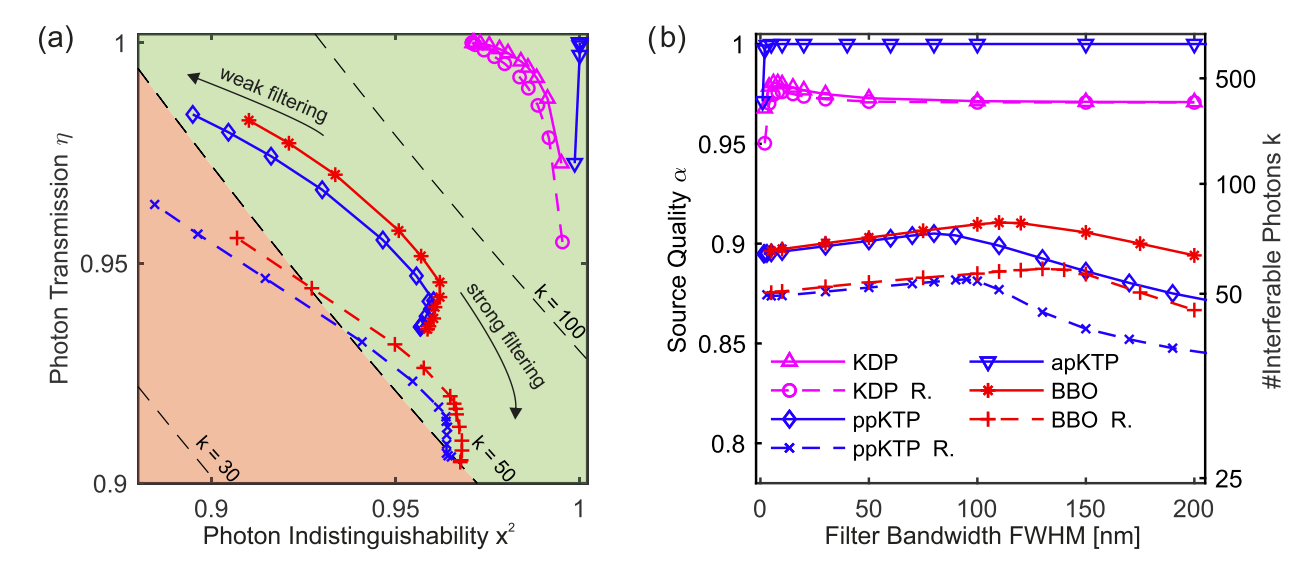
\includegraphics[scale=0.25]{pic/result1}
	\caption{(a)对应于不同晶体在不同滤波器带宽下的理想SPDC设置的每光子透射率$\eta$和不可分辨性$x^2$[参见(b)图例]. 虚线是等值线,表示一个玻色子采样实验可以使用多少光子k。
(b)对应光子数k(右轴)的值与滤波器带宽的函数。
在图例中后缀是R.为矩形滤波器,否则为高斯滤波器。}
	\label{fig:result1}
\end{figure}

我们用到的所有数据都在图\ref{fig:table}中。

\begin{figure}[ht]
	\centering
	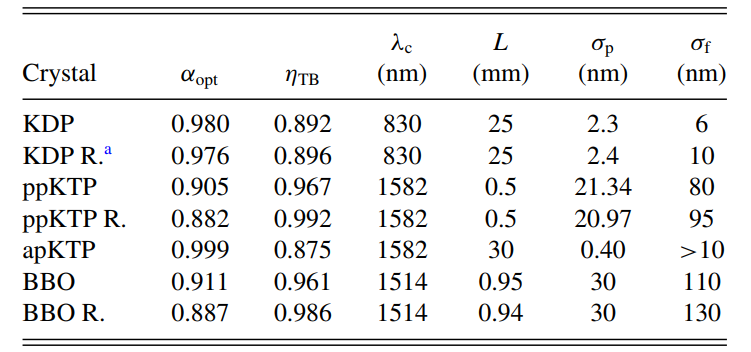
\includegraphics[scale=0.5]{pic/table}
	\caption{用到的数据}
	\label{fig:table}
\end{figure}

同样的道理,我们也可以模拟出谱纯度和滤波器带宽的关系,如图\ref{fig:result2}所示,值得一提的是,在滤波前(before filtering)谱纯度之所以下降是因为这个配置不再是可以因式分解的状态了,但这个机理可以在滤波后与滤波过程相互抵消,所以滤波之后会增加谱纯度。

同时图\ref{fig:result2}也解释了矩形滤波器窗口和高斯滤波器窗口的区别:

第一个不同之处在于,高斯滤波器允许较高的光子辐射值,因此在玻色子采样实验中会有更多的光子;

第二个区别是最优滤波器带宽。

这两种不同的解释是,矩形滤波窗口相对于高斯滤波窗口,只过滤了给定带宽,不含有其他值,所以允许通过的光子数更少。

\begin{figure}[ht]
	\centering
	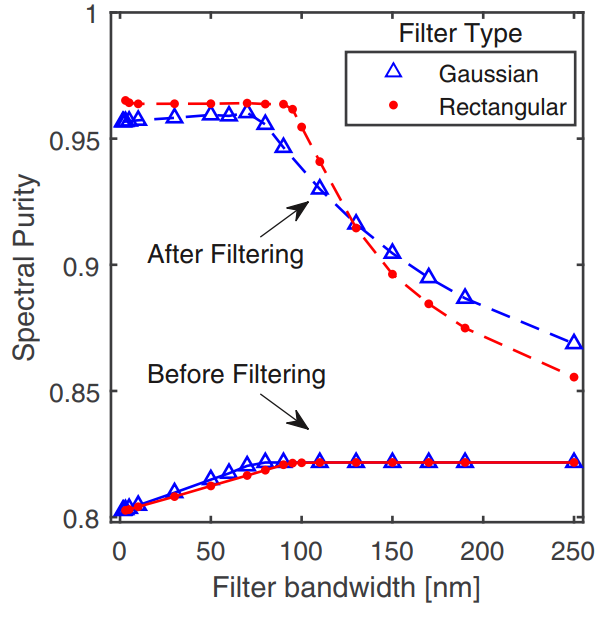
\includegraphics[scale=0.5]{pic/result2}
	\caption{具有sinc相位匹配函数的ppKTP源的光谱纯度。每个点都对应于这个滤波器源的最佳配置,这些源的纯度显示在过滤之前(实线)和之后(虚线).}
	\label{fig:result2}
\end{figure}

更进一步的,我们还可以画出滤波后的Joint Spectral Amplitude(JSA)的图\ref{fig:result3},它与JSI的关系是$JSI=\left|JSA\right|^2$.

\begin{figure}[ht]
	\centering
	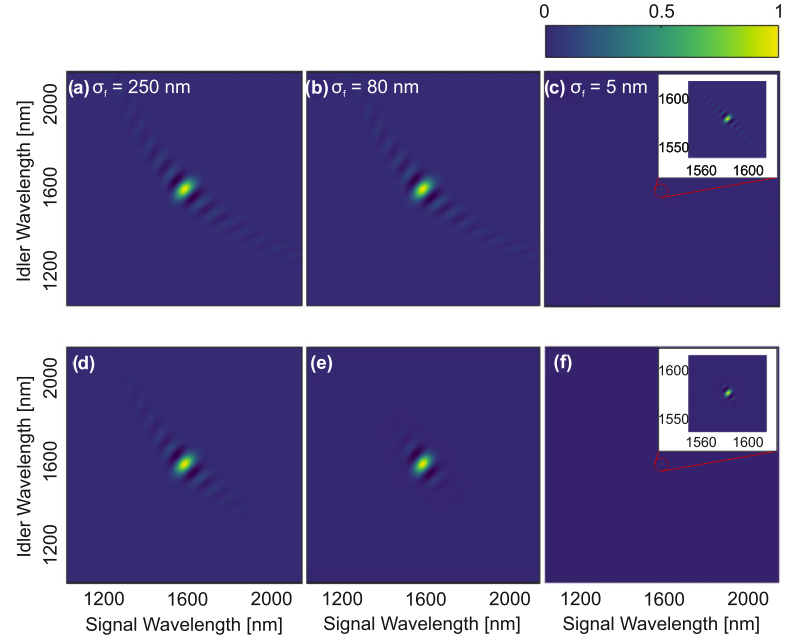
\includegraphics[scale=0.4]{pic/result3}
	\caption{ppKTP在其他条件最优化的情况下的JSA实部图。SPDC配置情况:弱滤波(左)、最优滤波(中)和强滤波(右)。上面三幅图表示过滤前,下面三幅图表示过滤后。}
	\label{fig:result3}
\end{figure}


并且经过我们进一步的计算,高斯变迹后的KTP源对附加损耗的有限容忍度表明,这个结果对波导源和大块源(bulk source)都是理想的。

\section{结论与讨论}

这篇文章通过数值模拟不同参数的SPDC光子源,从而找到每个非线性晶体对应的源质量的最大值,以论证可以用SPDC光子源实现量子优越性——即“量子霸权”。为了实现可以特定个光子的玻色取样实验,$\eta_{TB}=\frac{\alpha_{spe}}{\alpha_{opt}}$,我们只需要在现有的实验仪器条件下证明这个是可能的即可。

经过模拟计算,最好的晶体是apKTP,它的最大源质量可以达到$\alpha_{opt}=99\%$,这允许其他损失造成的透射率最小为$87\%$,而这个标准可以被现有的仪器实现;其次,KDP晶体也可以使源质量达到一个相对不错的值$\alpha_{opt}=98\%$. 

这表明,我们可以利用SPDC光子源来实现“量子霸权”(quantum supremacy),即:展示出量子计算机相对于经典超级计算机的优势。

最后,这篇文章的结果是在散射玻色子采样(scattershot boson sampling)的方案下模拟的,同样的操作可以推广到其他SPDC源比如四波混频或者高斯玻色取样的实验。

\section{我的感想}

从我自己一个量子光学学习者的观点来看,我认为本文给实现“量子优越性”提供了一个很方便的途径。因为现在科研界对于量子计算机的实现已经提出了很多方案,有的用LOQC,有的用原子离子,但哪一个方案能做出来第一个量子计算机?本文从理论的角度给出了其中一种量子计算机实现的可行性,这非常有意义!

因为我在李传锋老师的Cavity QED组里从事相关的实验,在实验过程中,我深深体会到用Cavity-Atom系统来实现量子优越性是非常难的。无论是冷原子的捕获与调控,还是腔的制作与对准,都需要克服巨大的技术问题。而且由于这种技术上的复杂,导致在实验室里很难大量复制这种系统。而在我读这篇文章,并从Boson Sampling的角度来考虑这个问题的时候,就像当年Aaronson和Arkhipov两人提出这个问题的时候,量子光学界科学家们的反应一样——我感觉非常妙绝。用这种方式证明“量子优越性”,确实是一个可以更加可行的办法。

其次,对非线性光学的调研与学习给我打开了一扇新的大门。我觉得非线性光学虽然计算比较复杂,但是物理图像比较有趣,比如差频产生、和频产生等。自然界中的非线性过程要远多于线性过程,而通过对非线性领域的学习,可以让人们利用更加多种多样的非线性过程来制造所需要的仪器设备(比如PPLN晶体),这是非常有意义并且有趣的。
 %这是正文

%----------------------------------------------------------------------------------------
%	REFERENCE LIST
%----------------------------------------------------------------------------------------

\phantomsection
\small
\renewcommand\refname{参考文献}
\bibliographystyle{unsrt}
\begin{thebibliography}{99}  

\bibitem{single_photon_source} Sinha, Urbasi et al. “Single photon sources: ubiquitous tools in quantum information processing.” arXiv: Quantum Physics (2019): n. pag.

\bibitem{REV} V A Reshetov. (2020) Photon emission by an atom with degenerate levels into a micro-cavity with polarization-degenerate mode. Laser Physics 30:8, pages 086001.

\bibitem{Scully}Scully, M., Zubairy, M. (1997). Quantum Optics. Cambridge: Cambridge University Press. doi:10.1017/CBO9780511813993

\bibitem{Geoffrey} New, G. (2011). Introduction to Nonlinear Optics. Cambridge: Cambridge University Press. doi:10.1017/CBO9780511975851

\bibitem{SPDC} Couteau, Christophe. “Spontaneous parametric down-conversion.” Contemporary Physics 59 (2018): 291 - 304.

\bibitem{Nonlinear_Crystall1}T. Kim, M. Fiorentino, and F. N. C. Wong, Phase-stable source of polarization-entangled photons using a polarization Sagnac interferometer, Phys. Rev. A 73, 012316 (2006).

\bibitem{Nonlinear_Crystall2}P. G. Kwiat, K. Mattle, H. Weinfurter, A. Zeilinger, A. V. Sergienko, and Y. Shih, New High-Intensity Source of Polarization-Entangled Photon Pairs, Phys. Rev. Lett. 75, 4337 (1995).

\bibitem{Nonlinear_Crystall3}P. J. Mosley, J. S. Lundeen, B. J. Smith, P. Wasylczyk, A. B. U’Ren, C. Silberhorn, and I. A. Walmsley, Heralded Generation of Ultrafast Single Photons in Pure Quantum States, Phys. Rev. Lett. 100, 133601 (2008).

\bibitem{Boson_Sampling} Gard, Bryan T. et al. “An Introduction to Boson-Sampling.” arXiv: Quantum Physics (2015): 167-192.

\bibitem{2011AA} S. Aaronson and A. Arkhipov, “The computational complexity of linear optics,” in Proc. 43rd Annu. ACM Symp. Theory of Comput., A. Press, Ed., pp. 333–342 (2011).

\bibitem{calculate_pemanent} L. Valiant, “The complexity of computing the permanent,” Theor. Comput. Sci. 8(2), 189–201 (1979).

\bibitem{theory_model} J. J. Renema, V. Shchesnovich, and R. Garcia-Patron, Classical simulability of noisy boson sampling, arXiv:1809.01953

\end{thebibliography}

%----------------------------------------------------------------------------------------

\end{document}